%% Preamble
  \documentclass{article}

  \usepackage[T1]{fontenc} % Use 8-bit encoding that has 256 glyphs
  \usepackage{fourier} % Use the Adobe Utopia font for the document - comment this line to return to the LaTeX default
  \usepackage[english]{babel} % English language/hyphenation
  \usepackage{amsmath,amsfonts,amsthm} % Math packages
  \usepackage{fancyhdr} % Required for custom headers
  \usepackage{lastpage} % Required to determine the last page for the footer
  \usepackage{extramarks} % Required for headers and footers
  \usepackage[pdftex]{graphicx}
  \usepackage{lipsum} % Used for inserting dummy 'Lorem ipsum' text into the template
  \usepackage{hyperref} % Used to add links to websites to the pdf
  \hypersetup{colorlinks,linkcolor=cyan,urlcolor=blue,citecolor=black}  % From Rick
  \usepackage{xifthen}
  \usepackage{booktabs}
  \usepackage{mdframed}

  % Margins
  \topmargin=-0.45in
  \evensidemargin=0in
  \oddsidemargin=0in
  \textwidth=6.5in
  \textheight=9.0in
  \headsep=0.25in

  \linespread{1.1} % Line spacing

  % Set up the header and footer
  \pagestyle{fancy}
  \lhead{\hmwkAuthorName} % Top left header
  \chead{\hmwkClass\ (\hmwkClassInstructor) \hmwkTitle} % Top center header
  \rhead{\firstxmark} % Top right header
  \lfoot{\lastxmark} % Bottom left footer
  \cfoot{} % Bottom center footer
  \rfoot{Page\ \thepage\ of\ \pageref{LastPage}} % Bottom right footer
  \renewcommand\headrulewidth{0.4pt} % Size of the header rule
  \renewcommand\footrulewidth{0.4pt} % Size of the footer rule
  \setlength\parindent{0pt} % Removes all indentation from paragraphs

  %%   DOCUMENT STRUCTURE COMMANDS
  % Header and footer for when a page split occurs within a problem environment
  \newcommand{\enterProblemHeader}[1]{
  \nobreak\extramarks{#1}{#1 continued on next page\ldots}\nobreak
  \nobreak\extramarks{#1 (continued)}{#1 continued on next page\ldots}\nobreak
  }

  % Header and footer for when a page split occurs between problem environments
  \newcommand{\exitProblemHeader}[1]{
  \nobreak\extramarks{#1 (continued)}{#1 continued on next page\ldots}\nobreak
  \nobreak\extramarks{#1}{}\nobreak
  }

  \setcounter{secnumdepth}{0} % Removes default section numbers
  \newcounter{homeworkProblemCounter} % Creates a counter to keep track of the number of problems

  \newcommand{\homeworkProblemName}{}
  \newenvironment{homeworkProblem}[1][Problem \arabic{homeworkProblemCounter}]{ % Makes a new environment called homeworkProblem which takes 1 argument (custom name) but the default is "Problem #"
  \stepcounter{homeworkProblemCounter} % Increase counter for number of problems
  \renewcommand{\homeworkProblemName}{#1} % Assign \homeworkProblemName the name of the problem
  \section{\homeworkProblemName} % Make a section in the document with the custom problem count
  \enterProblemHeader{\homeworkProblemName} % Header and footer within the environment
  }{
  \exitProblemHeader{\homeworkProblemName} % Header and footer after the environment
  }

  \newcommand{\problemAnswer}[1]{ % Defines the problem answer command with the content as the only argument
  \noindent \begin{mdframed} #1 \end{mdframed} % Makes the box around the problem answer and puts the content inside
  }

  \newcommand{\homeworkSectionName}{}
  \newenvironment{homeworkSection}[1]{ % New environment for sections within homework problems, takes 1 argument - the name of the section
  \renewcommand{\homeworkSectionName}{#1} % Assign \homeworkSectionName to the name of the section from the environment argument
  \subsection{\homeworkSectionName} % Make a subsection with the custom name of the subsection
  \enterProblemHeader{\homeworkProblemName\ [\homeworkSectionName]} % Header and footer within the environment
  }{
  \enterProblemHeader{\homeworkProblemName} % Header and footer after the environment
  }


  %   NAME AND CLASS SECTION
  \newcommand{\hmwkTitle}{Assignment\ \#2 - Statistics} % Assignment title
  \newcommand{\hmwkDueDate}{Tuesday,\ January\ 15,\ 2012} % Due date
  \newcommand{\hmwkClass}{Econ\ 588} % Course/class
  \newcommand{\hmwkClassInstructor}{McDonald} % Teacher/lecturer
  \newcommand{\hmwkAuthorName}{Spencer Lyon} % Your name

  %   TITLE PAGE
  \title{
      \vspace{2in}
      \textmd{\textbf{\hmwkClass:\ \hmwkTitle}}\\
      \normalsize\vspace{0.1in}\small{Due\ on\ \hmwkDueDate}\\
      \vspace{0.1in}\large{\textit{\hmwkClassInstructor}}
      \vspace{3in}
  }

  \author{\textbf{\hmwkAuthorName}}
  \date{} % Insert date here if you want it to appear below your name

% Add shortcut for some things I use alot (pdf's partial derivatives)
  \newcommand{\exppdf}[1]{%
    \ifthenelse{ \isempty{#1} }%
      {\ensuremath{\frac{e^{x/ \beta}}{\beta}}}% if #1 is empty
      {\ensuremath{\frac{e^{-#1/ \beta}}{\beta}}}% if #1 is not empty
  }

  \newcommand{\gampdf}[1]{%
    \ifthenelse{ \isempty{#1} }%
      {\ensuremath{\frac{x^{p-1} e^{-x / \beta}}{\beta^p \Gamma(p)}}}% if #1 is empty
      {\ensuremath{\frac{#1^{p-1} e^{-#1 / \beta}}{\beta^p \Gamma(p)}}}% if #1 is not empty
  }

  \newcommand{\fracpd}[2]{
    \ensuremath{\frac{\partial #1}{\partial #2}}
  }

  \newcommand{\ggpdf}[1]{%
    \ifthenelse{ \isempty{#1} }%
      {\ensuremath{ \frac{\left| a\right|  y^{a p-1} e^{-\left(\frac{y}{\beta}\right)^a}}{\beta ^{a p} \Gamma (p)}}}% if #1 is empty
      {\ensuremath{ \frac{\left| a\right|  #1^{a p-1} e^{-\left(\frac{#1}{\beta}\right)^a}}{\beta ^{a p} \Gamma (p)}}}% if #1 is not empty
  }

 \newcommand{\gbbpdf}[1]{%
    \ifthenelse{ \isempty{#1} }%
      {\ensuremath{ \frac{|a| y^{a p - 1}}{b^{a p} B(p, q)(1 + (y/b)^a)^{p+q}}}}% if #1 is empty
      {\ensuremath{ \frac{|a| #1^{a p - 1}}{b^{a p} B(p, q)(1 + (#1/b)^a)^{p+q}} }}% if #1 is not empty
  }

  \newcommand{\lognpdf}[1]{%
    \ifthenelse{ \isempty{#1} }%
      {\ensuremath{ \frac{1}{\sqrt{2 \pi } \sigma  x} e^{-\frac{(\log (x)-\mu )^2}{2 \sigma ^2}} }}% if #1 is empty
      {\ensuremath{ \frac{1}{\sqrt{2 \pi } \sigma  #1} e^{-\frac{(\log (#1)-\mu )^2}{2 \sigma ^2}} }}% if #1 is not empty
  }

  \newcommand{\multinpdf}[1]{%
    \ifthenelse{ \isempty{#1} }%
      {\ensuremath{ \frac{ e^{-\frac{1}{2} (y - \mu)' \Sigma^{-1} (y - \mu)} }{ (2 \pi)^{n/2} \left| \Sigma \right| ^{(1/2)}} }}% if #1 is empty
      {\ensuremath{ \frac{ e^{-\frac{1}{2} (#1 - \mu)' \Sigma^{-1} (#1 - \mu)} }{ (2 \pi)^{n/2} \left| \Sigma \right| ^{(1/2)}} }}% if #1 is not empty
  }

\begin{document}

% Problem 1
  \begin{homeworkProblem}
      \textbf{Show that the cumulative distribution function for the exponential is given by $$F(x:\theta)  = 1 - e^{-X/\beta} $$}
      \vspace{.2in}

      \problemAnswer{ % Answer
        The cdf can easily be obtained from the pdf by integrating the pdf from $0$ to $x$. I will show this below:

        \begin{align*}
            \int_0^X \frac{e^{-x/\beta} }{\beta} \mathrm{d}x = -e^{-x/\beta} \bigg|_{0}^X =-e^{-X/\beta} - \left(-e^{-0/\beta}  \right) = 1 - e^{-X/\beta} \qed
        \end{align*}
      }
  \end{homeworkProblem}

% Problem 2
  \begin{homeworkProblem}
      \textbf{Derive an expression for the hazard function for the exponential distribution.}
      \vspace{.2in}

      \problemAnswer{ % Answer
        The hazard function has the form $h(x) = \frac{f(x)}{1 - F(x)}$. I will derive the exponential distributions hazard function below:

        \begin{align*}
            h(x) = \frac{f(x)}{1 - F(x)} = \frac{\frac{e^{-x/\beta}} {\beta}}{1 - \left(1 - e^{-X/\beta} \right)}=\frac{e^{-x/ \beta}}{\beta \left(e^{-x / \beta} \right)} = \frac{1}{\beta} \qed
        \end{align*}
      }
  \end{homeworkProblem}

% Problem 3
  \begin{homeworkProblem}
      \textbf{Show that the moment generating function for the exponential distribution is given by $ \frac{1}{1 - \beta t}$}
      \vspace{.2in}

      \problemAnswer{ % Answer
        The moment generating function is given by the following expression $ M_t(x) = E[e^{tx}]$. I will derive this function below
        \begin{align*}
           M_t(x) = E[e^{tx}] = \int_0^{\infty} e^{tx} \frac{e^{-x/\beta} }{\beta} \mathrm{d}x= \frac{e^{\left(t x - \frac{x}{\beta}\right)}}{{\left(t - \frac{1}{\beta}\right)} \beta} \bigg|_{0}^{\infty} = -\frac{e^{- \infty (1 / \beta - t)}}{1 - \beta t} - \left(- \frac{e^{0}}{1 - \beta t} \right) = \frac{1}{1-\beta  t} \qed
        \end{align*}
      }
  \end{homeworkProblem}

% Problem 4
  \begin{homeworkProblem}
      \textbf{Write an expression for the cumulant generating function for the exponential distribution.}
      \vspace{.2in}

      \problemAnswer{ % Answer
        The cumulant generating function ($\Psi (t)$) is given by the taking the log of the moment generating function.
        \begin{align*}
            \Psi(t)  = \ln(M_t(x)) = \ln \left( \frac{1}{1 - \beta t}\right) = \ln(1) - \ln(1  -\beta t) = 0 - log(1 -\beta t) = - log(1 -\beta t) \qed
        \end{align*}
      }
  \end{homeworkProblem}

% Problem 5
  \begin{homeworkProblem}
      \textbf{Use the cumulant generating function for the exponential distribution to evaluate the following:}

      \begin{itemize}
        \item $E(x) = \mu = $
        \item $Var(x) = \sigma^2= $
        \item $E(x - \mu)^3 =  $
        \item $E(x - \mu)^4 =  $
      \end{itemize}

      \vspace{.2in}

      \problemAnswer{ % Answer
          To get the moments above we simply need to take the 1st, 2nd, 3rd, and 4th derivatives of the cumulant generating function above and evaluate at $t=0$.

          \begin{itemize}
            \item $E(x) = \mu = \frac{\partial \Psi(t)}{\partial t} = \frac{\partial (- log(1 -\beta t))}{\partial t} = \frac{\beta}{1 - \beta t} \bigg|_{t=0} = \beta$
            \item $Var(x) = \sigma^2 = \frac{\partial^2\Psi(t)}{\partial t^2} = \frac{\partial^2 (- log(1 -\beta t))}{\partial t^2} = \frac{\beta^2}{\left(1 - \beta \right)^2} \bigg|_{t=0} = \beta^2$
            \item $E(x - \mu)^3 = \frac{\partial^3\Psi(t)}{\partial t^3} = \frac{\partial^3 (- log(1 -\beta t))}{\partial t^3} = \frac{2 \beta^3}{\left(1 - \beta \right)^3} \bigg|_{t=0} = 2 \beta^3$
            \item  $E(x - \mu)^4  = \frac{\partial^4\Psi(t)}{\partial t^4} = \frac{\partial^4 (- log(1 -\beta t))}{\partial t^4} = \frac{6 \beta^4}{\left(1 - \beta \right)^4} \bigg|_{t=0} = 6 \beta^4$
          \end{itemize}

          \qed

      }
  \end{homeworkProblem}

% Problem 6
  \begin{homeworkProblem}
      \textbf{Show that the mode and median for the exponential distribution are given by 0 and (β ln 2), respectively.}
      \vspace{.2in}

      \problemAnswer{ % Answer
        The mode of a function is simply the most common or highest probability value. It is easy to see that the mode must be $x=0$ because the function is decreasing in x. Another way to write this is to say $$f(0) = \frac{e^{-0/\beta}}{\beta} > \frac{e^{-x/\beta}}{\beta} = f(x) \quad \forall x > 0$$

        We can easily solve for the median of the exponential distribution using this expression $\int_{-\infty}^X f(s) ds = 0.5$ and solving for $X$.

        \begin{align*}
            0.5 = \int_{-\infty}^X f(s) ds &= \int_0^X \frac{e^{-s/\beta}}{\beta}  ds \\
            &= -e^{-s/ \beta } \bigg|_0^X \\
            &= 1-e^{-X/ \beta } = 0.5 \\
            X &= \beta \ln(2) \qed
        \end{align*}
      }
  \end{homeworkProblem}

% Problem 7
  \begin{homeworkProblem}
      \textbf{Demonstrate that the MLE of β in the exponential distribution is given by $\tilde{\beta} = \bar{X} = \sum_{i=1}^N \left( \frac{X_i}{N} \right)$}
      \vspace{.2in}

      \problemAnswer{ % Answer
        The first step in solving this problem is to find the likelihood function. This is done for the exponential distribution as follows

        \begin{align*}
            L = \prod_{i=1}^N f(x_i) = \prod_{i=1}^N \exppdf{x_i} =\frac{e^{-\sum_{i=1}^N x_1/\beta}} {\beta^N}
        \end{align*}

        Once the likelihood function is found we need to find the log likelihood function $l(x) = \ln(L(x))$

        \begin{align*}
            l = \ln(L(x)) = \ln \left( \frac{e^{-\sum_{i=1}^N x_1/\beta}} {\beta^N} \right) = \sum_{i=1}^N \frac{x_i}{\beta} - n \ln(\beta)
        \end{align*}

        The final step is to take the derivative of the likelihood function, set it equal to zero, and solve for x:

        \begin{align*}
            0 = \fracpd{l}{\beta}  = \sum_{i=1}^N x_i \beta^{-2} - n \beta^{-1}  \rightarrow &{} \frac{\sum_{i=1}^N x_i}{N} = \tilde{\beta} \\ & \bar{x} = \tilde{\beta} \qed
        \end{align*}

        \qed

      }
  \end{homeworkProblem}

% Problem 8
  \begin{homeworkProblem}
      \textbf{The mgf for the gamma probability distribution ($f(x; p, b) = \gampdf{} $) is given by $\frac{1}{(1 - \beta t)^p}$. Show that the sum of n independent identically distributed exponential variables is distributed as $GA( ; \beta, p=n)$.}
      \vspace{.2in}

      \problemAnswer{ % Answer
        From equation (1.15) in the notes we have that the moment generating function for the sum of random variables is the product of the moment generating function for each of those random variables. In mathematical form this means that $M_{\sum_{i=1}^N X_i}(t) = \prod_{i=1}^N M_{X_i}(t)$.

        \vspace{.2in}
        We now need to find the moment generating function for the exponential distribution. This is found by the expression $E \left[ e^{tx} \right]$.

        \begin{align*}
            M_{exp}(t) = E \left[ e^{tx} \right] = \int_0^{\infty} \exppdf{} e^{xt} dx = \frac{e^{\frac{x (\beta  t-1)}{\beta }}}{\beta  t-1} \bigg |_0^{\infty} = 0 -  \frac{1}{\beta  t-1} = \frac{1}{1 - \beta t}
        \end{align*}

        Now that we have $M_{exp}(t)$ we can use the relation in the first paragraph of this solution to get the MGF for the sum of iid exponential random variables.

         \begin{align*}
            M_{\sum_{i=1}^N exp(\beta)}(t) = \prod_{i=1}^N M_{exp(\beta)}(t) = \prod_{i=1}^N  \frac{1}{1 - \beta t} = \left (  \frac{1}{1 - \beta t} \right) ^N= \frac{1}{\left( 1 - \beta t\right)^N}
        \end{align*}

        As shown in the problem description, this is the moment generating function for the gamma distribution with $\beta = \beta $ and $p = N $ $\qed$

      }
  \end{homeworkProblem}

% Problem 9
  \begin{homeworkProblem}
      \textbf{Using the results from question 8, demonstrate that the exact distribution of the sample mean $(Y)$ is given by GA$( ; \beta / n, p=n)$}
      \vspace{.2in}

      \problemAnswer{ % Answer
         First I formally define $\bar{Y} = \sum_{i=1}^N x_i$.I can then say that the sample mean of $\bar{Y}$ is the following (note that I define $T \equiv t / n$):

        \begin{align*}
            E\left[e^{\bar{Y} t}\right] = E\left[e^{ \left( \frac{1}{n}\right)\sum_{i=1}^N x_i t }\right] = E\left[e^{ \sum_{i=1}^N x_i T}\right] = \frac{1}{(1 - \beta T)^N} = \frac{1}{\left( 1 - \left( \frac{\beta}{n}\right) t\right)^N}
        \end{align*}

        As shown in problem 8 this is the moment generating function for a $GA (; \beta / n, n)$ distribution. \qed
      }
  \end{homeworkProblem}

% Problem 10
  \begin{homeworkProblem}
      \textbf{Consider a random sample $\{y_1, y_2, \dots, y_n \}$ where the density of $y_i$ is given by GG$(y_n; a, \beta, p)$ \\ (a) Form the log likelihood \\ (b) Obtain the MLE of $\beta$ for the case where $a = p = 1$, i.e., the exponential. \\ (c) Evaluate the second derivative of the log likelihood function with respect to $\beta$ for the exponential \\ (d) What is the asymptotic distribution of the MLE of $\beta$ for the exponential?}
      \vspace{.2in}

      \problemAnswer{ % Answer

        \homeworkSection{a.)}

        The pdf  of the generalized gamma distribution is given by $f(y; a, \beta, p)  = \ggpdf{}$. To find the log-likelihood function we need to first find the likelihood function $L = \prod_{i-1}^N f(y_i)$. Once we have that the log-likelihood function is just the natural log of the likelihood function.

        \begin{align*}
            l = \ln(L) = \ln \left( \prod_{i=1}^N \ggpdf{y_i} \right) = (ap - 1) \sum_{i=1}^N \ln(y_i) - \sum_{i=1}^N \left(\frac{y_i}{\beta} \right) ^a - n (ap) \ln(\beta) - N \ln (\Gamma(p))
        \end{align*}

        \homeworkSection{b.)}

        Now we were asked to obtain the MLE for $\beta$ in the case where $a = p = 1$. Under these conditions the log-likelihood function reduces to $$l = \sum_{i=1}^N \frac{x_i}{\beta} - n \ln(\beta)$$ To get the MLE we take the derivative of the log-likelihood function with respect to $\beta$, set it equal to 0, and solve for $\beta$. This is below.

        \begin{align*}
            0 = \fracpd{l}{\beta}  = \sum_{i=1}^N y_i \beta^{-2} - n \beta^{-1}  \rightarrow &{} \frac{\sum_{i=1}^N y_i}{N} = \tilde{\beta} \\ & \bar{y} = \tilde{\beta}
        \end{align*}

        \homeworkSection{c.)}

        The second derivative of the log-likelihood function for the exponential is given by the following

        \begin{align*}
            \fracpd{^2 l}{\beta^2} = -2 \sum_{i=1}^N y_i \beta^{-3} + n \beta ^{-2}
        \end{align*}

        \homeworkSection{d.)}

        The asymptotic distribution for the  MLE of $\beta$ for the exponential is $N(\beta, \beta^2 / n)$

        \qed
      }
  \end{homeworkProblem}

% Problem 11
  \begin{homeworkProblem}
      \textbf{The exact distribution of the sample mean of exponentially distributed variables is a gamma , GA $(z; \beta/n, p=n)$, (see problem 9) and the approximating "asymptotic" normal distribution is N$(z; \beta, \beta^2/n)$. The corresponding moment generating functions are given by: \\  \\ Gamma: $M_{GA} (t)= \frac{1}{\left(1 - \beta t \right)^n}$ \\ Normal: $M_N(t) = e^{\beta t + (t \beta)^2 / 2n}$ \\ \\ Compare the mean, variance, skewness, and kurtosis of the exact distribution and the approximating or asymptotic normal distribution.}
      \vspace{.2in}

      \problemAnswer{ % Answer
          To do this problem I need to know the cumulant generating function for the GA distribution. This is simply the natural log of the moment generating function.

          \begin{align*}
              \psi = \ln \left(\frac{1}{(1 - \beta t / n) ^ n} \right) = ln(1) = \ln(1) - n \ln(1  -\beta t / n) = 0 - n log(1 -\beta t / n) = - n log(1 -\beta t / n)
          \end{align*}

          I would have to do the same for the normal distribution, but I know what all these moments are from memory.

          \vspace{.15in}

              \begin{tabular}{l|c|c}
              \hline

              \hline
              \textbf{ } & \textbf{GA$( ; \beta / n, p=n)$} & \textbf{N($\mu = \beta, \sigma^2 = \beta^2 / n)$} \\
              \hline
                 Mean & $\beta$  & $\beta$ \\
                 Variance & $\beta^2 / n$\ & $\beta^2 / n$\\
                 Skewness & $\frac{2 \beta ^3}{n^2} \rightarrow \frac{2}{\sqrt{n}}$ & 0 \\
                 Kurtosis & $\frac{6 \beta ^4}{n^3} \rightarrow \frac{6}{n} $ & 3 \\
              \hline
              \end{tabular}

              \vspace{.15in}

               Note that the $\rightarrow$ in the Skewness and Kurtosis rows stands for division by $(\sigma^2)^{3/2}  \text{ and } (\sigma^2)^2$, respectively. \qed
          }

  \end{homeworkProblem}

% Problem 12
  \begin{homeworkProblem}
      \textbf{The Burr distribution and hazard functions \\ \\  (a) Demonstrate that GB2$(y; a, b, p=1, q) = \frac{|a| q(y/b)^{a-1)}}{b(1 + (y/b)^a)^{q+1}}$ \\ (b) Use these results to obtain an expression for the hazard function for the BR12. Recall that the hazard function is defined to be $\frac{pdf}{(1-cdf)}$ \\ (c) The hazard function for the Burr 12 with $a >1$ is upside down "U" shaped. Investigate the shape of the hazard function for the two cases (1) $0< a < 1$ and (2) $a = 1$. Assume that all parameter values are positive. Hint: What happens to thevalue of the hazard function as $y$ increases for arbitrarry but fixed values of $a$?}
      \vspace{.2in}

      \problemAnswer{ % Answer

        \homeworkSection{a.)}
        The pdf for the GB2 is $f(y) = \gbbpdf{}$. If we now set $p=1$ We can get what was asked for in part (a)

        \begin{align*}
            f(y;, 1, b, p=1, q) =\frac{|a| y^{a (1) - 1}}{b^{a(1)} B(1, q)(1 + (y/b)^a)^{1+q}} = \frac{|a| y^{a - 1}}{b^{a} (1/q) (1 + (y/b)^a)^{q}} = \frac{|a| q(y/b)^{a-1)}}{b(1 + (y/b)^a)^{q+1}}
        \end{align*}

        \homeworkSection{b.)}
        From the GB distribution tree we see that Burr12 = $GB2(y;1,b,=1,q)$, or the function we just derived. We are given the cdf for the Burr12, so to find the hazard function we just plug these objects into $h(y) = \frac{f(y)}{1 - F(y)}$.

        \begin{align*}
              h(y) = \frac{f(y)}{1 - F(y)} = \frac{\frac{|a| q(y/b)^{a-1)}}{b(1 + (y/b)^a)^{q+1}}} {1 - \left(1 - \left( \frac{1}{1 + (y/b)^a}\right)^q \right) } = \frac{q \left| a\right|  \left(\frac{y}{b}\right)^{a-1} \left(\frac{1}{\frac{y^2}{b^2}+1}\right)^{-q} \left(\left(\frac{y}{b}\right)^a+1\right)^{-q-1}}{b}
        \end{align*}

        \homeworkSection{c.)}

        When $ 0 < a < 1$, the hazard function is U shaped. This means that as y increases so does the value of the hazard function. With $a = 1$ The function is still U shaped, but less so. See Figure ~\ref{fig:b12Haz}.

        \qed

      }
      \begin{figure}[!h]
        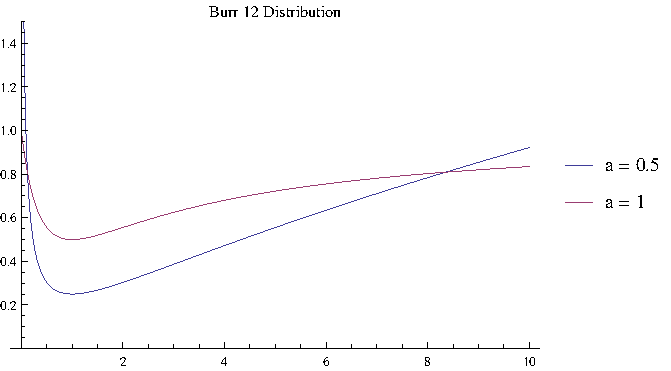
\includegraphics[width=\linewidth, height=4in]{Graphics/b12Haz.pdf}
        \caption{Hazard function for the Burr 12 distribution with 2 different values for $a$ and $b = q = 1$.}
        \label{fig:b12Haz}
      \end{figure}


  \end{homeworkProblem}

% Problem 13
  \begin{homeworkProblem}
      \textbf{What are the possible shapes of the hazard function for the gamma, Weibull and exponential and distributions? (Hint: This problem is not requesting a derivation. Refer to figure 4 for the generalized gamma function).}
      \vspace{.2in}

      \problemAnswer{ % Answer

        \begin{itemize}
            \item For the Gamma distribution, when $p < 1$, the shape is decreasing, and when $p >1$ the shape increasing
            \item The Weibull distribution hazard function is increasing when $ a > 1$ and decreasing when $ a < 1$
            \item For the exponential distribution, the hazard function can only be constant
        \end{itemize}

        \qed

      }
  \end{homeworkProblem}

% Problem 14
  \begin{homeworkProblem}
      \textbf{If $Y \sim LN(\mu, \sigma^2)$, verify that $Z = Y^2 \sim LN(2\mu, 4\sigma^2)$. Don't forget the Jacobian in your analysis of the transformation.}
      \vspace{.2in}

      \problemAnswer{ % Answer
        The pdf of the lognormal distribution is $f(x; \mu, \sigma) = \lognpdf{}$. To solve for the distribution of $Z$ I need to apply the transformation equation $h(z) = f(g^{-1}(z) = y) \left|\fracpd{y}{z} \right|$

        \begin{itemize}
            \item $z = y^2 \rightarrow y = \sqrt(z)$
            \item $\fracpd{y}{z} = \frac{1}{2 \sqrt{y}}$
            \item $f(g^{-1}(z)) = \lognpdf{\sqrt{z}} $
            \item $h(z) = \lognpdf{\sqrt{z}}  \frac{1}{2 \sqrt{z}} = \frac{1}{2 z \sigma \sqrt{2 \pi} } e^{- \frac{(1/2 \log(z) - \mu)^2}{2 \sigma^2}} = \frac{1}{2 z \sigma \sqrt{2 \pi} } e^{- \frac{ (1/4) (\log(z) - 2 \mu)^2}{2 \sigma^2}} =  \frac{e^{-\frac{(\log (z)-2 \mu )^2}{8 \sigma ^2}}}{2 \sqrt{2 \pi } \sigma z} $
            \item The above is distributed $LN(2 \mu, 4 \sigma^2) $
        \end{itemize}

        \qed
      }
  \end{homeworkProblem}

% Problem 15
  \begin{homeworkProblem}
      \textbf{If $X \sim GA(x; \beta = 1, p)$, verify that $Y = \beta X^{1/a} \sim GG(y ; a, \beta, p)$. Don't forget the Jacobian in your analysis of the transformation.}
      \vspace{.2in}

      \problemAnswer{ % Answer
        The pdf for this gamma distribution is $f(x; \beta = 1, p) = \frac{x^{p-1} e^{-x }}{\Gamma(p)}$. We will repeat the procedure from the previous problem

        \begin{itemize}
            \item $y = \beta x^{1/a} \rightarrow x = \left( \frac{y}{\beta} \right) ^ a$
            \item $\fracpd{x}{y} = \frac{a \left(\frac{y}{\beta }\right)^{a-1}}{\beta }$
            \item $f(g^{-1}(y)) = \frac{e^{-\left(\frac{y}{\beta }\right)^a} \left(\left(\frac{y}{\beta }\right)^a\right)^{p-1}}{\Gamma (p)} $
            \item $h(y) = \frac{e^{-\left(\frac{y}{\beta }\right)^a} \left(\left(\frac{y}{\beta }\right)^a\right)^{p-1}}{\Gamma (p)} \left(  \frac{a \left(\frac{y}{\beta }\right)^{a-1}}{\beta }\right) = \frac{a e^{-\left(\frac{y}{\beta }\right)^a} \left(\left(\frac{y}{\beta }\right)^a\right)^p}{y \Gamma (p)} $
            \item The above is distributed $GG(y; a, \beta, p)$.
        \end{itemize}

        \qed
      }
  \end{homeworkProblem}

% Problem 16
  \begin{homeworkProblem}
      \textbf{Use the cumulant generating function for the normal, $N(\mu, \sigma^2)$, to show that the normalized or scaled kurtosis for a normally distributed random variable is given by 3.}
      \vspace{.2in}

      \problemAnswer{ % Answer
        The cumulant generating function for the normal distribution is $ \psi_N = \frac{\sigma ^2 t^2}{2}+\mu  t$. To find the normaled or scaled kurtosis I just need to evaluate the expression $\fracpd{^4 \psi_N}{t^4} \bigg|_{t=0} / \left[(\sigma^2)^2 \right]$

        \begin{itemize}
            \item $\fracpd{\psi_N}{t} = \mu + \sigma^2 t$
            \item $\fracpd{^2 \psi_N}{t^2} =  \sigma^2 t$
            \item $\fracpd{^3 \psi_N}{t^3} = 0$
            \item $\fracpd{^4 \psi_N}{t^4} = 0$
        \end{itemize}

        Excess Kurtosis is defined as  $E(X - E(X))^4 - 3 (\text{Variance})^2$. It is also true that the excess kurtosis is equal to $\fracpd{^4 \psi_N}{t^4}$. From above we know that $\fracpd{^4 \psi_N}{t^4} = 0$ and we can then solve for scaled kurtosis.

        \begin{align*}
            \fracpd{^4 \psi_N}{t^4} = 0 = E(X - E(X))^4 - 3 (\text{Variance})^2 = E(X - E(X))^4 - 3 (\sigma^2)^2
        \end{align*}

        \begin{align*}
            E(X - E(X))^4 =3 (\sigma^2)^2 \rightarrow \frac{E(X - E(X))^4}{\sigma^4} = 3 \qed
        \end{align*}
      }
  \end{homeworkProblem}

% Problem 17
  \begin{homeworkProblem}
      \textbf{Given that the $n x 1$ vector $Y$ is distributed as $N(\mu, \Sigma)$, where $\Sigma$ is positive definite, demonstrate that the mode of the univariate density $N(\mu, \Sigma)$ occurs at $Y = \mu$. This means demonstrate $\fracpd{f(Y)}{Y} \bigg|_{Y=\mu} = 0 $ and note that $\frac{\partial ^2 f(Y)}{Y^2}$ is negative definite.}
      \vspace{.2in}

      \problemAnswer{ % Answer
        The pdf for the multivariate normal distribution is given by $f = \multinpdf{}$. I will begin be expanding the exponent in this expression

        \begin{align*}
            f(y) = \multinpdf{} = \frac{ e^{-\frac{1}{2} \left[ y' \Sigma^{-1} y - y' \Sigma^{-1} \mu - \mu' \Sigma^{-1} y + \mu' \Sigma^{-1} \mu \right]} }{ (2 \pi)^{n/2} \left| \Sigma\right|^{(1/2})}
        \end{align*}

        I will now take the first and second derivatives of this function with respect to $y$.

        \begin{itemize}
            \item $\fracpd{f(y)}{y} = - \frac{1}{2} \left[ 2 \Sigma^{-1} y - \Sigma^{-1} \mu - \mu' \Sigma^{-1} \right] \multinpdf{}$
            \item $\fracpd{^2f(y)}{y^2} = - \frac{1}{2} \left[ 2 \Sigma^{-1} \right] \multinpdf{}$
         \end{itemize}

         I will now evaluate the first derivative at $y = \mu$

         \begin{align*}
            \fracpd{f(y)}{y} \bigg|_{y = \mu} = - \frac{1}{2} \left[ 2 \Sigma^{-1} \mu - \Sigma^{-1} \mu - \mu' \Sigma^{-1} \right] \multinpdf{\mu} = 0 \frac{e^0}{(2 \pi)^{n/2} \left| \Sigma\right|^{(1/2}} = 0
         \end{align*}

         The first condition in the problem description has been satisfied, it remains to show that $\fracpd{^2f(y)}{y^2}$ is negative definite. Because $\Sigma$  is positive definite, so is $\Sigma^{-1}$. The quadratic form in the numerator is also positive definite because it is around the matrix $\Sigma^{-1}$. Finally, the denominator is just constants and the determinant of $\Sigma$. That determinant is positive because all the characteristic roots of $\Sigma$ are positive. This means the entire expression is guaranteed to be negative because of the $-\frac{1}{2}$ in front. \qed
      }
  \end{homeworkProblem}

% Problem 18
  \begin{homeworkProblem}
      \textbf{Given $g(X) = 2x_1^2 + (5/2)x_2^2 + 4x_1x_2 + x_1 + 3x_2$ \\ \\ (a) Demonstrate that $g(X) =\left(\begin{smallmatrix} x_1 & x_2 \end{smallmatrix}\right)\left(\begin{smallmatrix} 2 & 2 \\ 2 & 5/2 \end{smallmatrix}\right) \left(\begin{smallmatrix} x_1 \\ x_2 \end{smallmatrix}\right)$ \\ (b)  Use the technique of differentiating $g(X)$ with respect to the vector $X = \left(\begin{smallmatrix} x_1 & x_2 \end{smallmatrix}\right)$', determine the vector $X$ which is associated with an optimum of $g(X)$ \\ (c) Evaluate $\frac{\partial^2 g(X)}{\partial X^2}$ and determine whether your answer to (b) corresponds to a maximum or a minimum}
      \vspace{.2in}

      \problemAnswer{ % Answer
        \homeworkSection{a.)}
        To demonstrate part (a) I will just expand out the part we are given and show that it is equivalent to the quadratic form we started with.

        \begin{align*}
            \left(\begin{smallmatrix} x_1 & x_2 \end{smallmatrix}\right) \left(\begin{smallmatrix} 2 & 2 \\ 2 & 5/2 \end{smallmatrix}\right) \left(\begin{smallmatrix} x_1 \\ x_2 \end{smallmatrix}\right)  + \left(\begin{smallmatrix} x_1 & x_2 \end{smallmatrix}\right)  \left(\begin{smallmatrix} 1 \\ 3 \end{smallmatrix}\right) = \left(\begin{smallmatrix} x_1 & x_2 \end{smallmatrix}\right) \left(\begin{smallmatrix} 2 x_1+2 x_2 \\ 2 x_1+\frac{5 x_2}{2} \end{smallmatrix}\right) + x_1 + 3 x_2 = 2x_1^2 + (5/2)x_2^2 + 4x_1x_2 + x_1 + 3x_2
        \end{align*}

        \homeworkSection{b.)}

        The derivative of the quadratic form is $\fracpd{g(X)}{X} = 2\left(\begin{smallmatrix} 2 & 2 \\ 2 & 5/2 \end{smallmatrix}\right) \left(\begin{smallmatrix} x_1 \\ x_2 \end{smallmatrix}\right)  + \left(\begin{smallmatrix} 1 \\ 3 \end{smallmatrix}\right)$. To find the optimum I will set this equal to zero and solve for $X$.

        \begin{align*}
             - \left(\begin{smallmatrix} 1 \\ 3 \end{smallmatrix}\right) = 2\left(\begin{smallmatrix} 2 & 2 \\ 2 & 5/2 \end{smallmatrix}\right) \left(\begin{smallmatrix} x_1 \\ x_2 \end{smallmatrix}\right) = \left(\begin{smallmatrix} 4 & 4 \\ 4 & 5 \end{smallmatrix}\right) \left(\begin{smallmatrix} x_1 \\ x_2 \end{smallmatrix}\right)
        \end{align*}

        \begin{align*}
            - \left(\begin{smallmatrix} 5/4 & -1 \\ -1 & 1 \end{smallmatrix}\right) \left(\begin{smallmatrix} 1 \\ 3 \end{smallmatrix}\right)= \left(\begin{smallmatrix} 5/4 & -1 \\ -1 & 1 \end{smallmatrix}\right) \left(\begin{smallmatrix} 4 & 4 \\ 4 & 5 \end{smallmatrix}\right) \left(\begin{smallmatrix} x_1 \\ x_2 \end{smallmatrix}\right) = \text{I} \left(\begin{smallmatrix} x_1 \\ x_2 \end{smallmatrix}\right)
        \end{align*}

        \begin{align*}
            \left(\begin{smallmatrix} x_1 \\ x_2  \end{smallmatrix}\right) = \left(\begin{smallmatrix}  7/4 \\ -2 \end{smallmatrix}\right)
        \end{align*}

        \homeworkSection{c.)}
        Now I will look at second order conditions: $\fracpd{^2G(X)}{X^2} = \left(\begin{smallmatrix} 4 & 4 \\ 4 & 5 \end{smallmatrix}\right)$. It can be shown that the eigen values for this matrix are $ \frac{1}{2} (9 \pm \sqrt{65})$, which are both positive. This means the matrix is positive definite and the optimum I found was a minimum. \qed
      }
  \end{homeworkProblem}

% Problem 19
  \begin{homeworkProblem}
      \textbf{Let $i = \{1, 1, \dots, 1 \}$' \\ \\ (a) Evaluate $i'i$ \\ (b) Evaluate $ii'$ \\ (c) Demonstrate that the matrix $\left( \frac{1}{n} ii' \right)$ is symmetric and idempotent}
      \vspace{.2in}

      \problemAnswer{ % Answer
        Without loss of generality I assume that $i$ has $n$ elements. In this situation the answers are:

        \begin{itemize}
          \item $i'i = n$
          \item $ii' = \left(\begin{smallmatrix} 1 & 1 & \dots & 1 \\ 1 & 1 & \dots & 1 \\  \vdots & \vdots & \ddots & \vdots \\ 1& 1 &\dots& 1 \end{smallmatrix}\right)$, where its shape is $n x n$.
          \item The matrix $\left( \frac{1}{n} ii' \right)$ is obviously symmetric because every element is exactly the same (in this case each element is equal to $\frac{1}{n}$). This matrix is idempotent because $\left( \frac{1}{n} ii' \right) \left( \frac{1}{n} ii' \right) = \frac{1}{n^2} i(i'i)i' = \frac{1}{n^2} i (n) i' = \frac{1}{n} ii'$
        \end{itemize}

         \qed

      }
  \end{homeworkProblem}

% Problem 20
  \begin{homeworkProblem}
      \textbf{Let $y_i$ be iid as $N(0, \sigma ^2)$ or in other words $Y \sim N(0, \sigma^2 I_n)$ \\ \\
      (a) Determine the distribution of $\bar{Y}  = \sum_{t=1}^n \frac{y_t}{n}$ \\
      (b) Demonstrate that $A$ is idempotent. \\
      (c) Verify that trace$(A) = n - 1$ \\
      (d) Demonstrate that the distribution of $s^2(n-1) / \sigma^2$ is $\chi^2(n-1)$ \\
      (e) Verify that $Y$ and $s^2$ are independently distributed \\
      (f) What is the distribution of $\left( \frac{\frac{\bar{Y} - 0 }{\sigma /n}}{\left(\frac{s^2(n-1)}{\sigma^2} / (n-1) \right)^{1/2} } \right) = \frac{\bar{Y} - 0}{s / n}$ ?}
      \vspace{.2in}

      \problemAnswer{ % Answer
      \homeworkSection{a.)}
        The first 'useful theorem' states that if $Y \sim N(\mu, \Sigma)$, then $Z = AY \sim(B \mu, B\Sigma B')$.  Using this theory it is easy to see that $\bar{Y} \sim N((\frac{1}{n}) i' \mu_y, (\frac{1}{n} )i' \Sigma_Y (\frac{1}{n} )i) = N(0, (\frac{\sigma^2}{n^2}) i'i)$

        \homeworkSection{b.)}

        We are given the following:

        \begin{align*}
            s^2 = \sum (y_i - \bar{Y})^2 / (n - 1) = \dots = \frac{Y'AY} {(n-1)}, \quad \text{ where } A = I - \frac{1}{n} ii'
        \end{align*}

        To show that $A$ is idempotent we simply need to show that $AA = A$. I do this below

        \begin{align*}
            AA &= \left( I - \frac{1}{n} ii' \right) \left( I - \frac{1}{n} ii'\right) \\
            &= II - \frac{1}{n} I ii' - \frac{1}{n}ii' I + \frac{1}{n^2} (ii')(ii') \\
            &= I - \frac{2}{n} - \frac{1}{n^2} n ii' \\
            &= I - \frac{2}{n} ii' - \frac{1}{n} ii' \\
             &= I - \frac{1}{n} ii'
        \end{align*}

        \homeworkSection{c.)}

        Because the $Tr(A)$ is the sum of the diagonal entries, it is going to be equal to $n (1) - \left(\frac{1}{n} \right) (n (1)) = n - 1$. The first part comes from $I$ and the second part comes from the fact that every entry of ($\left( \frac{1}{n} \right) ii'$) is equal to $\left( \frac{1}{n}\right)$.

        \homeworkSection{d.)}

        On to part d: Let $\hat{s} \equiv s^2 (n-1) / \sigma^2 = \left(\frac{Y'AY}{(n-1)}\right) \frac{(n-1)}{\sigma^2} = Y'AY / \sigma^2$. The 2nd useful theorem says that if $Y \sim N(0, I)$ and $A$ is a symmetric idempotent matrix, then $Y'AY \sim \chi^2(m)$, where m is equal to $Tr(A)$. We don't quite have that, but if you remember $Y \sim N(0, \sigma^2 I)$, so you when you take into account the $\left(\frac{1}{\sigma^2} \right)$ in $\hat{s}$, we can cancel the $\sigma^2$ terms and we can apply the 2nd useful theorem. We have shown that $A$ is idempotent and it is clearly symmetric. We have also shown that the $Tr(A) = n - 1$, therefore $\hat{s} \sim \chi^2(n -1)$

        \homeworkSection{e.)}

        For part e we will appeal to the 4th useful theorem, which states that if $Y \sim N(0, I)$ and L is a ($kxn$) matrix of rank $k$, then $LY$ and the idempotent quadratic form $Y'AY$ are independently distributed if $LA = 0$. In the context of our problem, $A = I - \left(\frac{1}{n} \right) ii'$ and $L = \left( \frac{1}{n} \right) i'$. We can now apply this theorem =:

        \begin{align*}
            AL &= \left[  I - \left(\frac{1}{n} \right) ii' \right] \left[ \left( \frac{1}{n} \right) i' \right] \\
            &= I \left( \frac{1}{n} \right) i' - \left(\frac{1}{n} \right) ii' \left( \frac{1}{n} \right) i'\\
            &= \left( \frac{1}{n} \right) i' - \left( \frac{1}{n^2}\right) n i' \\
            &= \left( \frac{1}{n} \right) i' - \left( \frac{1}{n} \right) i' \\
            &= 0
        \end{align*}

        \homeworkSection{f.)}

        From point (4) of the distribution theory for the normal we learn that $\frac{N(0, 1)}{\sqrt{\chi^2(d) / d}} \sim t(d)$. Applying this to our problem, we already know that $\left(\frac{s^2(n-1)}{\sigma^2} / (n-1) \right)^{1/2}  = \sqrt{\chi^2(n - 1) / (n-1)}$. This is the denominator of the relation from point (4).  We also know that $\bar{Y} \sim N(0, \left( \frac{\sigma^2}{n^2}\right) i'i$, which means that $\frac{\bar{Y}}{\sigma / n} = \frac{\bar{Y - 0}n}{\sigma} \sim N\left(\frac{n}{\sigma} 0, \left( \frac{n^2}{\sigma^2} \right) \left( \frac{\sigma^2}{n^2} \right) i'i \right) = N(0, i'i)$. This is analogous to the $N(0, 1)$ in the numerator for part (4) of the distribution theory section. All of this means that $\frac{\bar{Y} - 0}{s /n} \sim t(n - 1)$. \qed

      }
  \end{homeworkProblem}

% Problem 21
  \begin{homeworkProblem}
      \textbf{The mean and variance of a Gamma are given by $\beta p \text{ and } \beta^2 p$, respectively. Let the corresponding sample moments by denoted by $\bar{Y} \text{ and } s^2$ \\ \\ (a) Derive the method of moments estimators of the parameters $\beta \text{ and } p$ \\ (b) Derive the method of moments estimator of the parameter $\beta$ in an exponential distribution. \\ (c) Using two sample moments discuss how you could use the generalized method of moments estimation to estimate the parameter $\beta$ in an exponential distribution.}
      \vspace{.2in}

      \problemAnswer{ % Answer
        \homeworkSection{a}

        To use the method of moments you simply set the theoretical moments equal to the sample moments and solve for parameters. Doing that in this case gives this system of two equations: $\bar{Y} = \beta p \text{ and } s^2 = \beta^2 p$. I will solve them below by making the substitution $p = \frac{\bar{Y}}{\beta}$

        \begin{align*}
            s^2 = \beta^2 p = \beta ^2 \frac{\bar{Y}}{\beta} = \beta \bar{Y} \rightarrow \hat{\beta} = \frac{s^2}{\bar{Y}}
        \end{align*}

        \begin{align*}
          \hat{p} = \frac{\bar{Y}}{\beta} = \frac{\bar{Y}}{s^2 / \bar{Y}} = \left(\frac{\bar{Y}}{s} \right) ^2
        \end{align*}

        \homeworkSection{b}

        The MOM estimator for $\beta$ in an exponential distribution is just $\hat{\beta} = \bar{Y}$

        \homeworkSection{c}

        To use GMM we need to create a vector function $g(\theta)$ that is simply equal to the difference between each sample moment and its theoretical counterpart. We would then solve the optimization problem $\min_{\theta} g(\theta)' W g(\theta)$, where $W$ is some weighting matrix. For example, if you wanted to place equal importance on each moment $W$ would be the identity matrix. \\

        To do this for the exponential distribution, we would say that $g(\theta) = \left(\begin{smallmatrix} (\bar{Y} - \beta) & (s^2 - \beta^2) \end{smallmatrix}\right)$. The optimal $W$ in this case is found by the expression $W^{-1} = \text{Var}(g(\theta))$.


      }
  \end{homeworkProblem}

  \begin{table}[ht]
  \begin{center}
    \begin{tabular}{c|r|l}
    \toprule
      a & b & c\\
      \midrule
      $1$ & $2$ & $3$\\
      $4$ & hello & $\infty$\\
    \bottomrule
    \end{tabular}
  \end{center}
\end{table}

\begin{table}[ht]
\begin{center}
  \begin{tabular}{ccc}
  \toprule
  ab & b & c\\
   \midrule
  1 & 2 & 3.0\\
  4 & hello & inf\\
  \bottomrule
  \end{tabular}
\end{center}
\end{table}


\begin{table}[ht]
  \begin{center}
    \begin{tabular}{|ccc|}
    \toprule
      ab & b & c\\
      \midrule
      $1$ & $2$ & $3$\\
      $4$ & hello & $\infty$\\
    \bottomrule
    \end{tabular}
  \end{center}
\end{table}

\begin{table}[ht]
  \begin{center}
    \begin{tabular}{rccc}
    \toprule
       & ab & b & c\\
      \midrule
      A & $1$ & $2$ & $3$\\
      B & $4$ & hello & $\infty$\\
    \bottomrule
    \end{tabular}
  \end{center}
\end{table}

\begin{table}[ht]
  \begin{center}
    \begin{tabular}{rccc}
    \toprule
       & ab & b & c\\
      \midrule
      A & $1$ & $2$ & $3$\\
      B & $4$ & hello & $\infty$\\
    \bottomrule
    \end{tabular}
  \end{center}
\end{table}

\end{document}
